\documentclass[brazil, a4paper, 11pt]{article}

% --- PREÂMBULO ---
% 1. Load 'Universal' Toolkit (Project-Agnostic)
% █▀█ █▀█ █▀▀ ▄▀█ █▀▄▀█ █▄▄ █   █▀▀
% █▀▀ █▀▄ ██▄ █▀█ █ ▀ █ █▄█ █▄▄ ██▄

% NOTE: The packages (and related commands) in this preamble are loaded following the bellow ordering.
% Packages related to:
	% 1. Document canvas (i.e.: page geometry);
	% 2. Typeface system (i.e.: used fonts);
	% 3. Document structure (i.e.: headers formatting);
	% 4. Floats (i.e.: non-textual elements);
	% 5. Micro-Layout (i.e.: "inline" adjustments);
	% 6. Finalization (i.e.: packages best loaded last).

%::::::::::::::::::::::::::::::::::::::::::::::::::::::::::::::::::::::::::::::::
%                                   1. CANVAS                                    
%           Define document's physical space plus some basic utilities           
%................................................................................
% CANVAS
\usepackage[
	a4paper,
	margin = 2cm,
]{geometry}			% Set page geometry
\usepackage[brazil]{babel}	% Adjust document to the language it's written in

% BASIC UTILITIES
\usepackage{csquotes}		% Language-sensitive quoting;
				% 'csquotes' works in tandem with 'babel'
\usepackage[dvipsnames]{xcolor}	% Access to 68 named colors
\usepackage{moresize}		% Additional font sizes
\usepackage[normalem]{ulem}	% More underline styles (and aligns bottoms of multiple underlines)
				% 'normalem' prevents underlines from altering \emph


%::::::::::::::::::::::::::::::::::::::::::::::::::::::::::::::::::::::::::::::::
%                               2. TYPEFACE SYSTEM                               
%    Define all fonts - for text, algorithms and math - used in the document     
%................................................................................
% 2.1 SYSTEM BACKEND
\usepackage{fontspec}		% Native Unicode-to-OpenType mapping;
				% Replaces legacy TeX font-enconding hacks;
				% DOCUMENT MUST NOW BE COMPILED WITH Lua OR XeLaTex

\usepackage{amsmath}		% AMS's package for mathematical typesetting
\usepackage{mathtools}		% Extends amsmath's functionalities (i.e.: a superset)
\usepackage[
	math-style = ISO,
	bold-style = ISO
]{unicode-math}			% Must be loaded after 'mathtools';
				% DOCUMENT MUST NOW BE COMPILED WITH Lua OR XeLaTex

%. . . . . . . . . . . . . . . . . . . . . . . . . . . . . . . . . . . . . . . . . 
% 2.2 SYSTEM DEFINITION
% 2.2.1 TEXT FONTS
\setmainfont{Tex Gyre Pagella}[Scale = 1.0]
\setsansfont{URW Classico}[
	Scale = MatchLowercase,	% Ensure main and sans fonts are at the same scale
]
\setmonofont{Inconsolata}[Scale=MatchLowercase]

% 2.2.2 MATH FONTS
\setmathfont{Libertinus Math}[Scale=MatchLowercase]
% Manually pick distinct calligraphic (Chancery hand) and script (Round hand) fonts for a greater variety of symbols
\setmathfont{XITS Math}[
	Scale 		= MatchLowercase,
	range		= {cal,bfcal},
	StylisticSet	= 1
]
\setmathfont{Libertinus Math}[
	Scale 		= MatchLowercase,
	range		= {scr,bfscr}
]
% Define a custom font face 'mathopfont' and use it to distinguish mathematical operators from prose
\setmathfontface\mathopfont{Latin Modern Roman}[Scale=MatchLowercase]
\setoperatorfont\mathopfont


%::::::::::::::::::::::::::::::::::::::::::::::::::::::::::::::::::::::::::::::::
%                             3. DOCUMENT STRUCTURE                              
%  Article or book-like structure assumed. Here, we just stylise their headers   
%................................................................................
\usepackage{titlesec}		% Controls vertical rhithm and heading aesthetics
\usepackage[titles]{tocloft}	% Change ToC fonts to match chosen heading aesthetics
\usepackage{appendix}		% Manages back-matter structure

% STYLISE HEADINGS
\ifdefined\part
	\titleformat{\part}[display]
		{\sffamily\bfseries\huge\filcenter}	% Format
		{\MakeUppercase{\partname}\ \thepart}	% Label
		{1em}					% Space between number and title
		{\Huge\MakeUppercase}			% Before-code
\fi
\ifdefined\chapter
	\titleformat{\chapter}[display]
		{\sffamily\bfseries\Large}			% Format
		{\MakeUppercase{\chaptertitlename}\ \thechapter}% Label
		{1em}						% Space between number and title
		{\huge\MakeUppercase}				% Before-code
\fi
\titleformat{\section}
    {\sffamily\bfseries\large}	% Format
    {\thesection}		% Label
    {1em}			% Space between number and title
    {\MakeUppercase}		% Before-code
\titleformat{\subsection}
    {\sffamily\bfseries}	% Format
    {\thesubsection}    	% Label
    {1em}               	% Space between number and title
    {\MakeUppercase}    	% Before-code
\titleformat{\subsubsection}
    {\sffamily\bfseries\small}	% Format
    {\thesubsubsection}		% Label
    {1em}               	% Space between number and title
    {\MakeUppercase}    	% Before-code
\titleformat{\paragraph}[runin]
    {\sffamily\bfseries}	% Format
    {\theparagraph}		% Label
    {1em}			% Space between number and title
    {}				% Before-code
\titlespacing*{\paragraph}
    {0pt}			% Left margin indentation
    {3.25ex plus 1ex minus .2ex}% Space BEFORE the paragraph title (vertical)
    {1em}			% Space AFTER the title (horizontal)

%. . . . . . . . . . . . . . . . . . . . . . . . . . . . . . . . . . . . . . . . . 
% 3.2 STYLISE HEADINGS IN ToC SPECIFICALLY
% Set the font for Table of Contents entries to Sans-Serif
\ifdefined\part
	\renewcommand{\cftpartfont}{\sffamily\bfseries}
	\renewcommand{\cftpartpagefont}{\sffamily\bfseries}
\fi
\ifdefined\chapter
	\renewcommand{\cftchapfont}{\sffamily\bfseries}
	\renewcommand{\cftchappagefont}{\sffamily\bfseries}
\fi
\renewcommand{\cfttoctitlefont}{\sffamily\bfseries\large\MakeUppercase}
\renewcommand{\cftsecfont}{\sffamily\bfseries}
\renewcommand{\cftsecpagefont}{\sffamily\bfseries}
\renewcommand{\cftsubsecfont}{\sffamily}
\renewcommand{\cftsubsecpagefont}{\sffamily}
\renewcommand{\cftsubsubsecfont}{\sffamily}
\renewcommand{\cftsubsubsecpagefont}{\sffamily}

%. . . . . . . . . . . . . . . . . . . . . . . . . . . . . . . . . . . . . . . . . 
%\usepackage{fancyhdr}		% Custom headers and footers
%\pagestyle{plain}	% header: empty; footer: centered page number


%::::::::::::::::::::::::::::::::::::::::::::::::::::::::::::::::::::::::::::::::
%                                    4. FLOATS                                   
%               Manage Floating Content (e.g.: figures and tables)               
%................................................................................
% FLOATS IN GENERAL
\usepackage{float}	% Provides [H] 'Here' float placement specifier (use with caution)
\usepackage{subcaption}	% Format multiple images (tables) in one figure (table) environment
			% NOTE: This package *automatically* loads the 'caption' package,
\captionsetup{
	labelfont = {small,bf},
	textfont  = {small,it}
}
%\subcaptionsetup{...}	% Uncomment to customize sub-captions separately

%. . . . . . . . . . . . . . . . . . . . . . . . . . . . . . . . . . . . . . . . . 
% TABLES
\usepackage{booktabs}	% Format tables following scientific convention
\usepackage{multirow}	% Allow multirow cells in tables

%. . . . . . . . . . . . . . . . . . . . . . . . . . . . . . . . . . . . . . . . . 
% IMAGES
% NATIVE PROGRAMMATIC DIAGRAMS & PLOTS
\usepackage{tikz}		% Create vector graphics programmatically
\usetikzlibrary{arrows.meta}	% Additional arrow styles
\usetikzlibrary{calc}		% Coordinate calculations
\usetikzlibrary{positioning}	% Better relative placement of notes
\usepackage{pgfplots}		% Tool for creating function plots and charts
\pgfplotsset{compat=1.18}	% Enforce version 1.18 for consistency

% EXTERNAL IMAGE MANAGEMENT
\usepackage{graphicx}		% LaTeX standard for including external image files

%. . . . . . . . . . . . . . . . . . . . . . . . . . . . . . . . . . . . . . . . . 
% ALGORITHMS
\usepackage[
	portuguese,
	ruled,
	vlined,
	linesnumbered
]{algorithm2e}	% Typeset formal algorithms
% Set algorithm font to the chosen monospace font
\SetAlFnt{\small\ttfamily}
\SetAlCapFnt{\small\ttfamily}
% Define Portuguese keywords
\SetKwInput{KwRequer}{Requer}
\SetKwInput{KwPrecondicao}{Pré-condição}
\SetKwInput{KwInicializa}{Inicializa}
\SetKwFor{Para}{para}{faça}{fim para}
\SetKwIF{Se}{SenaoSe}{Senao}{se}{então}{senão se}{senão}{fim se}
\DontPrintSemicolon


%::::::::::::::::::::::::::::::::::::::::::::::::::::::::::::::::::::::::::::::::
%                             5. MICRO-LAYOUT                              
%                       Packages that alter "inline" text                        
%................................................................................
% TEXT
\usepackage{multicol}		% Environment with multiple columns of text
\usepackage{enumitem}		% Customize list environments (provides 'resume')

%. . . . . . . . . . . . . . . . . . . . . . . . . . . . . . . . . . . . . . . . . 
% Now... for the micro-layout good stuff...
%
% █▀▄▀█ ▄▀█ ▀█▀ █ █
% █ ▀ █ █▀█  █  █▀█
%
% NICHE MATH PACKAGES
\usepackage{xfrac}	% Slanted fractions (\sfrac)
\usepackage{cancel}	% Strike-through for symbols (\cancel and \cancelto)
\usepackage{amsthm}	% AMS's package for creating theorem-like environments

%::::::::::::::::::::::::::::::::::::::::::::::::::::::::::::::::::::::::::::::::::
%                         5.1 CUSTOM THEOREM ENVIRONMENTS                          
%                                   (Colour-coded)                                  
%..................................................................................
% DEFINE COLOUR CODE FOR EACH THEOREM-LIKE ENVIRONMENT;
% (makes changing the colour choice effortless!)
\colorlet{lmm}{DarkOrchid}	% For lemma env.
\colorlet{thm}{Tan}		% For theorem env.
\colorlet{prop}{Maroon}		% For proposition env.
\colorlet{crl}{RawSienna}	% For corollary env.
\colorlet{def}{OliveGreen}	% For definition env.
\colorlet{eg}{RoyalPurple}	% For example env.
\colorlet{ex}{RoyalPurple}	% For exercise env.
\colorlet{obs}{MidnightBlue}	% For remark env.
\colorlet{note}{PineGreen}	% For notation remark env.

%. . . . . . . . . . . . . . . . . . . . . . . . . . . . . . . . . . . . . . . . . 
% DEFINE CUSTOM THEOREM STYLES
% > STYLE I - TAUTOLOGIES - FIRST NUMBER, THEN NAME
\newtheoremstyle{number-name}
{4mm}						% Space above env.
{4mm}						% Space below env.
{\itshape}					% Body font
{}						% Indent amount
{\bfseries}					% Head font
{:}						% Punctuation after head
{.3em}						% Space after head
{\thmnumber{#2}\,\thmname{#1}\thmnote{ (#3)}}	% Head spec

% > STYLE II - EXAMPLES & EXERCISES - FIRST NAME, THEN ITALIC NUMBER 
\newtheoremstyle{name-it_number}
{4mm}						% Space above env.
{4mm}						% Space below env.
{\itshape}					% Body font
{}						% Indent amount
{\bfseries}					% Head font
{}						% Punctuation after head
{.3em}						% Space after head
{\thmname{#1}\,{\itshape\thmnumber{#2}}}	% Head spec

% > STYLE III - REMARKS, SOLUTIONS & PROOFS - NO NUMBERING (should refer to a numbered env.)
\newtheoremstyle{no_number}
{4mm}						% Space above env.
{4mm}						% Space below env.
{}						% Body font
{}						% Indent amount
{\bfseries\itshape}				% Head font
{.}						% Punctuation after head
{.3em}						% Space after head
{}						% Head spec

% > STYLE IV - NOTATION REMARKS - NO NUMBERING (should refer to a numbered env.) AND ITALIC BODY 
\newtheoremstyle{no_number-it_body}
{4mm}						% Space above
{4mm}						% Space below
{\itshape}					% Body font
{}						% Indent amount
{\bfseries}					% Head font
{:}						% Punctuation after head
{.3em}						% Space after head
{}						% Head spec

%. . . . . . . . . . . . . . . . . . . . . . . . . . . . . . . . . . . . . . . . .
% APPLY THEOREM STYLES AND DEFINE RESPECTIVE ENVIRONMENTS
% > STYLE I - TAUTOLOGIES - FIRST NUMBER, THEN NAME
\theoremstyle{number-name}
  \newtheorem{lemma}{\color{lmm}Lema}[section]
  \newtheorem{theorem}{\color{thm}Teorema}[section]
  \newtheorem{proposition}{\color{prop}Proposição}[section]
  \newtheorem{corollary}{\color{crl}Corolário}[section]
  \newtheorem{definition}{\color{def}Definição}[section]

% Manually force counters to share the 'lemma' counter (i.e.: shared counter for style I)
\makeatletter
	\let\c@theorem\c@lemma
	\let\c@proposition\c@lemma
	\let\c@corollary\c@lemma
	\let\c@definition\c@lemma
\makeatother

% > STYLE II - EXAMPLES & EXERCISES - FIRST NAME, THEN ITALIC NUMBER 
\theoremstyle{name-it_number}
  \newtheorem{exercise}{\textcolor{ex}{Exercício}}[section]
  \newtheorem{example}{\textcolor{eg}{Exemplo}}[section]

% Manually force 'example' to use the 'exercise' counter (i.e. shared counter for style II)
\makeatletter
\let\c@example\c@exercise
\makeatother

% > STYLE III - REMARKS, SOLUTIONS & PROOFS - NO NUMBERING
\theoremstyle{no_number}
  % Remark
  \newtheorem*{observation*}{\color{obs}Observação}
  % Solution
  \newtheorem*{solution}{\color{ex}Solução}
  % Proofs
  \newtheorem*{proofT}{\color{thm}Demonstração}
  \newtheorem*{proofL}{\color{lmm}Demonstração}
  \newtheorem*{proofC}{\color{crl}Demonstração}
  \newtheorem*{proofP}{\color{prop}Demonstração}
  \newtheorem*{proofE}{\color{eg}Demonstração}
  \newtheorem*{proofO}{\color{obs}Demonstração}

% > STYLE IV - NOTATION REMARKS - NO NUMBERING AND ITALIC BODY 
\theoremstyle{no_number-it_body}
  \newtheorem*{notation*}{\color{note}Notação}

%. . . . . . . . . . . . . . . . . . . . . . . . . . . . . . . . . . . . . . . . .
% EXTRA: CUSTOM QED SYMBOL (a small 'black square' U+25A0)
\renewcommand\qedsymbol{■}


%:::::::::::::::::::::::::::::::::::::::::::::::::::::::::::::::::::::::::::::::::
%                            5.2 CUSTOM MATH COMMANDS                             
%.................................................................................
\newcommand{\Bvec}[1]{\symbf{#1}}	% Bold symbol vector notation

% CONSTANTS
\newcommand{\e}{\symup{e}}	% ISO notation for Euler's number
\newcommand{\im}{\symup{i}}	% ISO notation for the imaginary unit
\newcommand{\piup}{\symup{\pi}}	% ISO notation for pi

% RELATIONS
\newcommand{\longto}{\longrightarrow}	% Alias to note function domain/codomain (f: A --> B)

% Below, a colon-equals (and an analogous equals-colon) sign built 'from scratch', to be more compact and elegant
\newcommand*{\Defeq}{%
	\mathrel{%				% Wrapper so TeX treats/interprets the symbol as a relation
		\vcenter{%			% Vertically center the 'colon' part
			\baselineskip0.5ex%	% Manually set the vertical spacing between the dots
			\lineskiplimit0pt%	% Disable TeX's 'anti-collision' rule for full control
			\hbox{\scriptsize.}%	% The top dot
			\hbox{\scriptsize.}%	% The bottom dot
		}%
		{=}%				% The equals sign
	}%
}					% Compact colon-equals
\newcommand*{\Eqdef}{%
	\mathrel{%				% Wrapper so TeX treats/interprets the symbol as a relation
		{=}%				% The equals sign
		\vcenter{%			% Vertically center the 'colon' part
			\baselineskip0.5ex%	% Manually set the vertical spacing between the dots
			\lineskiplimit0pt%	% Disable TeX's 'anti-collision' rule for full control
			\hbox{\scriptsize.}%	% The top dot
			\hbox{\scriptsize.}%	% The bottom dot
		}%
	}%
}					% Compact equals-colon
\newcommand{\subnormal}{\triangleleft}	% Normal subgroup (left)
\newcommand{\supnormal}{\triangleright}	% Normal subgroup (right)

% UNARY OPERATIONS
\newcommand{\T}{{\symsfup{T}}}	% Transpose symbol
\newcommand{\Tp}[1]{{#1}^{\T}}	% Transpose operation

% OPERATORS
\newcommand{\diff}{\mathop{}\!\symup{d}}% Differential operator (with spacing)
\DeclareMathOperator{\dist}{dist}
\DeclareMathOperator{\map}{map}

% LOGIC
\newcommand{\limplies}{\rightarrow}	% Conditional connector
\newcommand{\liff}{\leftrightarrow}	% Biconditional connector
\newcommand{\nand}{\uparrow}		% NAND connector
\newcommand{\nor}{\downarrow}		% NOR connector
\newcommand{\xor}{\veebar}		% XOR connector


%:::::::::::::::::::::::::::::::::::::::::::::::::::::::::::::::::::::::::::::::::
%                                  FINALIZATION                                   
%                 Packages that patch others. MUST BE LOADED LAST                 
%.................................................................................
% BIBLIOGRAPHY                                   
\usepackage[
	backend	= biber,	% Use Biber backend (more powerful than BibTex)
	style	= ieee,
	backref	= true
]{biblatex}

%. . . . . . . . . . . . . . . . . . . . . . . . . . . . . . . . . . . . . . . . .
% HYPERLINKS
\usepackage{hyperref}	% Add hyperlinks to references, ToC and URLs
\hypersetup{
	plainpages	= false,	% Attempts to prevent duplicate page anchors
	colorlinks	= true,		% true: colored links; false: boxed links
	linkcolor	= NavyBlue,	% Internal links
	citecolor	= NavyBlue,
	urlcolor	= NavyBlue,
	breaklinks	= true,
	pdfborder	= {0 0 0}
}

%. . . . . . . . . . . . . . . . . . . . . . . . . . . . . . . . . . . . . . . . .
% REFERENCING
\usepackage[
	brazilian,
	nameinlink
]{cleveref}	% \cref is objectively better than \autoref

% DEFINE 'cleveref' NAMES FOR CUSTOM THEOREM-LIKE ENVIRONMENTS
	% STYLE I ENVIRONMENTS
\crefname{lemma}{lema}{lemas}
\Crefname{lemma}{Lema}{Lemas}
\crefname{theorem}{teorema}{teoremas}
\Crefname{theorem}{Teorema}{Teoremas}
\crefname{proposition}{proposição}{proposições}
\Crefname{proposition}{Proposição}{Proposições}
\crefname{corollary}{corolário}{corolários}
\Crefname{corollary}{Corolário}{Corolários}
\crefname{definition}{definição}{definições}
\Crefname{definition}{Definição}{Definições}
	% STYLE II ENVIRONMENTS
\crefname{exercise}{exercício}{exercícios}
\Crefname{exercise}{Exercício}{Exercícios}
\crefname{example}{exemplo}{exemplos}
\Crefname{example}{Exemplo}{Exemplos}

\newcommand{\customref}[2]{%	% Simple alias for custom link text
	\hyperref[#2]{#1}%
}

%. . . . . . . . . . . . . . . . . . . . . . . . . . . . . . . . . . . . . . . . .
% MICRO-TYPOGRAPHY
\usepackage{microtype}		% Enhance micro-typography (e.g.: protrusion, expansion)
				% Loaded last for best compatibility with other packages


% 2. Configure Project-Specific File Paths & Metadata
% 2.1. File Paths
%\addbibresource{bibliografia.bib}
\graphicspath{ {../output/} }

% 2.2. Metadata
%\hypersetup{
%	pdftitle={},
%	pdfauthor={}
%}

% 3. Load Packages Specific to this Document's Structure (if any)
\renewcommand{\arraystretch}{1.5}

% --- INÍCIO DO DOCUMENTO ---
\begin{document}
	% --- TÍTULO ---
	\begin{center}
	\rule{0.95\textwidth}{1.5pt}

	
	{\sffamily SME\,0221 Introdução à Inferência Estatística}

	\vspace*{.5\baselineskip}

	{\sffamily Trabalho Prático}

	\vspace*{1.25\baselineskip}

	{\sffamily\bfseries\Large\MakeUppercase{Estatística Descritiva}}
	
	\vspace*{1.5\baselineskip}

	\begin{tabular}{lcr}
		Cody Stefano Barham Setti & -- & 4856322 \\
		Vinícius de Sá Ferreira & -- & 15491650
	\end{tabular}

	\vspace*{1.5\baselineskip}
	
	{\normalsize 16 de Abril de 2026}

	\vspace*{.5\baselineskip}

	{\normalsize São Carlos, SP, Brasil}


	\rule{0.95\textwidth}{1.5pt}
\end{center}


	% --- CORPO DO TEXTO ---
	\noindent
	Da plataforma de competições de ciência de dados \textit{Kaggle} --- uma subsidiária da \textit{Google} --- extraímos o banco de dados \verb|titanic.csv|, que contém uma série de informações sobre 891 passageiros do infame Titanic.

	Para nosso trabalho, contudo, focamos em apenas três dados de cada passageiro:
	\begin{enumerate}
		\item sexo (``feminino'' ou ``masculino'');
		
		\item idade, em anos;

		\item preço de seu bilhete, em libras esterlinas (\pounds).
	\end{enumerate}
	Consideramos para nossos cálculos apenas passageiros sem dados faltantes. Portanto, restringimo-nos a 714 deles.
	Ao se tratar da modelagem que fizemos de cada conjunto de dados:
	\begin{enumerate}
		\item Os valores ``feminino'' e ``masculino'' não são quânticos nem ordenáveis. Portanto, interpretamos os sexos dos passageiros como amostragens de uma \textbf{variável qualitativa nominal}.

		\item Arredondamos as idades\footnote{As idades sofreram ``arredondamento bancário'', especificamente.} a anos inteiros --- já que algumas são registradas de forma fracionária no arquivo \verb|titanic.csv|. Logo, após o arredondamento, interpretamos as idades como amostragens de uma \textbf{variável quantitativa discreta}.

		\item No momento de venda, em 1912, os bilhetes do Titanic foram cobrados no sistema monetário \textit{Sterling} antigo, com valores dados em libras, xelins e pence. Todavia, no banco de dados \verb|titanic.csv| --- disponibilizado no \emph{Kaggle} em 2012 --- estes valores foram convertidos ao novo sistema \textit{Sterling}, de 1971 em diante. Portanto, cada valor é dado por um único número de libras, embora seja frequentemente um número fracionário. Com isso em mente, interpretamos os preços como amostragens de uma única \textbf{variável quantitativa contínua}.
	\end{enumerate}
	\vspace*{\baselineskip}
	
	\noindent\textbf{a) Com base no rol, calcular a média, mediana e moda e compare-as}
	\begin{table}[H]
		\centering
		\caption{Medidas de posição dos conjuntos de dados}
		\begin{tabular}{c|ccc}
			\toprule
						& Sexo		& Idade (anos)	& Preço (\pounds)	\\
			\midrule
			$\bar{X}$	& -			& 29,69			& 34,69 			\\
			Md			& -			& 28,00			& 15,74 			\\
			Mo			& masculino	& 24,00			& 13,00				\\
			\bottomrule
		\end{tabular}
	\end{table}
	\vspace*{2\baselineskip}

	\noindent\textbf{b) Com base no rol, calcular os quartis, interpretando-os}

	\begin{table}[H]
		\centering
		\caption{Quartis das idades e dos preços dos bilhetes dos passageiros\footnotemark}
		\begin{tabular}{c|cc}
			\toprule
					& Idade (anos)	& Preço (\pounds)	\\
			\midrule
			$Q_1$	& 20			& 8,05 				\\
			$Q_2$	& 28			& 15,74 			\\
			$Q_3$	& 38			& 33,25				\\
			\bottomrule
		\end{tabular}
	\end{table}
	\footnotetext{Quartis de índices fracionários foram calculados pela média simples dos dois valores de índices mais próximos.}
	Ao analisarmos os quartis das idades, observamos que 25\% dos passageiros tinham até 20 anos ($Q_1$), enquanto 75\% da amostra possuía idade igual ou inferior a 38 anos ($Q_3$). A mediana ($Q_2$) indica que metade dos passageiros tinha no máximo 28 anos, evidenciando uma concentração de jovens adultos na embarcação.

	Quanto aos preços dos bilhetes, a disparidade econômica torna-se evidente: enquanto 25\% dos passageiros pagaram até \pounds\,$8,05$ ($Q_1$), a mediana ($Q_2$) revela que metade do grupo desembolsou no máximo \pounds\,$15,74$ por sua passagem. O terceiro quartil ($Q_3$) mostra que 75\% dos passageiros pagaram até \pounds\,$33,25$, valor que, embora superior aos demais quartis, ainda é drasticamente inferior ao valor máximo de \pounds\,$512,33$. Essa proximidade entre $Q_1$, $Q_2$ e $Q_3$ em relação à amplitude total reforça a existência de uma grande massa de passageiros com bilhetes de baixo custo frente a uma minoria com passagens de luxo.
	\vspace*{2\baselineskip}
	
	\noindent\textbf{c) Calcular a amplitude total, amplitude interquartílica, o desvio-padrão e coeficiente de variação. Ressaltar dentre as variáveis quantitativas qual tem maior variabilidade}
	\begin{table}[H]
		\centering
		\caption{Medidas de dispersão dos conjuntos de dados quantitativos}
		\begin{tabular}{c|cc}
			\toprule
					& Idade (anos)	& Preço (\pounds)	\\
			\midrule
			$A$		& 80,00			& 512,33			\\
			$d_Q$	& 18,00			& 25,20 			\\
			$S$		& 14,52			& 52,92				\\
			$CV(\%)$& 48,92			& 152,53			\\
			\bottomrule
		\end{tabular}
	\end{table}
	O coeficiente de variação dos preços é maior do que o das idades e, portanto, a variável associada aos preços possui variabilidade maior do que a associada às idades.
	\vspace*{2\baselineskip}

	\noindent\textbf{d) Com a comparação das medidas de tendência central, avaliar a simetria}
	\vspace*{0.5\baselineskip}

	Tanto no caso das idades, quanto no caso dos preços, a mediana é inferior à média. Portanto, ambos os conjuntos possuem assimetria à direita.
	\vspace*{2\baselineskip}
	
	\noindent\textbf{e) Sumarizar as informações em tabela}
	\vspace*{0.5\baselineskip}

	Para sumarizar as informações relativas a sexo, como apenas duas categorias foram registradas, optamos por uma tabela de frequência simples.
	\begin{table}[H]
		\centering
		\caption{Frequência de sexos}
		\begin{tabular}{c|c}
			\toprule
			Sexo		& Frequência\\
			\midrule
			Feminino	& 261		\\
			Masculino	& 453		\\
			\bottomrule
		\end{tabular}
	\end{table}
	Para as idades e os preços, todavia, que são muitos, optamos por tabelas de frequência por classes. Para as idades, as classes elegidas foram décadas. Para os preços, elegemos 11 classes de mesma amplitude, conforme sugere a regra de Sturges.
	\begin{table}[H]
		\begin{minipage}[t]{0.48\textwidth}
			\centering
			\caption{Frequência de idades por década}
			\begin{tabular}{c|c}
				\toprule
				Faixa Etária (anos)& Frequência\\
				\midrule
				$0\vdash 10$	& 62		\\
				$10\vdash 20$	& 102		\\
				$20\vdash 30$	& 220		\\
				$30\vdash 40$	& 167		\\
				$40\vdash 50$	& 89		\\
				$50\vdash 60$	& 48		\\
				$60\vdash 70$	& 19		\\
				$70\vdash 80$	& 6			\\
				$80\vdash 90$	& 1			\\
				\bottomrule
			\end{tabular}
		\end{minipage}
		\hfill
		\begin{minipage}[t]{0.48\textwidth}
			\centering
			\caption{Frequência de preços de bilhetes por classes}
			\begin{tabular}{c|c}
				\toprule
				Preço (\pounds)		& Frequência\\
				\midrule
			    $  0,000\vdash 46,575$	& 566	\\
				$ 46,575\vdash 93,151$	& 98	\\
				$ 93,151\vdash 139,726$	& 22	\\
				$139,726\vdash 186,302$	& 10	\\
				$186,302\vdash 232,877$	& 7		\\
				$232,877\vdash 279,452$	& 8		\\
				$279,452\vdash 326,028$	& 0		\\
				$326,028\vdash 372,603$	& 0		\\
				$372,603\vdash 419,178$	& 0		\\
				$419,178\vdash 465,754$	& 0		\\
				$465,754\vdash 512,842$	& 3		\\
				\bottomrule
			\end{tabular}
		\end{minipage}
	\end{table}
	\vspace*{\baselineskip}

	\noindent\textbf{f) Com base nas informações tabeladas, calcular a média, mediana, moda, os quartis e o desvio-padrão. Compare os valores das medidas obtidas com o rol.}
	\begin{table}[H]
		\centering
		\caption{Medidas reconstruídas a partir das tabelas de frequência}
		\begin{tabular}{c|ccc}
			\toprule
						& Sexo		& Idade (anos)	& Preço (\pounds)	\\
			\midrule
			$\bar{X}$	& -			& 30,25			& 40,90 			\\
			Md			& -			& 25,00			& 23,29 			\\
			Mo			& masculino	& 25,00			& 23,29				\\
			$Q_1$		& -			& 25,00			& 23,29				\\
			$Q_2$		& -			& 25,00			& 23,29				\\
			$Q_3$		& -			& 35,00			& 23,29				\\
			$S$			& -			& 14,97			& 48,91				\\
			\bottomrule
		\end{tabular}
	\end{table}
	Primeiramente, como o sexo dos passageiros foi tabelado seguindo frequências simples, não há perda de informações, ou seja, as estatísticas devem permanecer idênticas. Pelo outro lado, como a variável associada é qualitativa nominal, ela apresenta uma única estatística: sua moda.

	Por sua vez, ao se tratar das estatísticas relativas à idade dos passageiros e ao preço de seus bilhetes, a começar, vemos que as médias reconstruídas estão deslocadas à direita das originais, mas os valores são próximos.

	Tanto para a idade dos passageiros, quanto para o preço  de seus bilhetes, há uma classe significativamente mais frequente do que todas outras, $20 \vdash 30$ anos e \pounds\,$0$ $\vdash$ \pounds\,$46,575$, respectivamente. Para o preço, em particular, essa diferença de frequência é gritante.

	Consequentemente, a mediana, a moda e os quartis desses dados convergem ao ponto médio de tal classe, $25$ anos ou \pounds\,$23,29$. Para a idade, este efeito não é tão forte, afinal, $Q_3 = 35$ anos, o ponto médio da classe seguinte. Mas, para o preço, todos quartis reconstruídos coincidiram em \pounds\,$23,29$.

	Por fim, o desvio padrão das idades aumentou muito ligeiramente, ao passo que o dos preços diminui ligeiramente. Acreditamos que a diminuição --- no caso dos preços --- deve-se ao fato de preços, antes próximos, agora serem valorados no preço idêntico de \pounds\,$23,29$.
	\vspace*{2\baselineskip}
	
	\noindent\textbf{g) Sumarizar as informações de cada variável graficamente (apresente dois gráficos), interpretando-as. Para a variável quantitativa contínua, apresentar obrigatoriamente o histograma e o \textit{boxplot}}.
	\begin{figure}[H]
		\centering
		\begin{subfigure}[t]{.49\textwidth}
			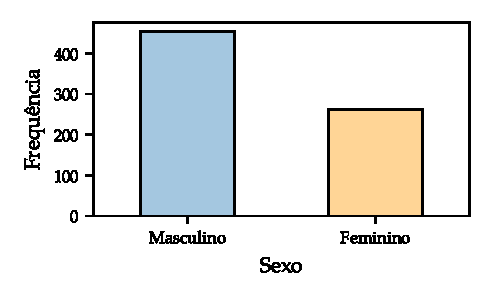
\includegraphics[width=\linewidth]{sexo_barra.pdf}
			\caption{Gráfico de barras}
		\end{subfigure}
		\hfill
		\begin{subfigure}[t]{.49\textwidth}
			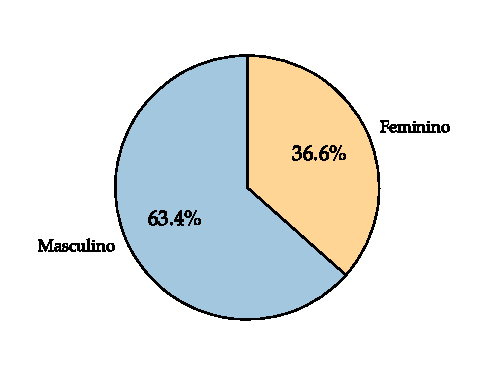
\includegraphics[width=\linewidth]{sexo_pizza.pdf}
			\caption{Gráfico de setores}
		\end{subfigure}
		\caption{Gráficos relativos aos sexos dos passageiros}
	\end{figure}
	Ambos os gráficos, mas, em especial, o de setores, mostram que a tripulação masculina do Titanic era próxima do dobro da feminina. Ou, ao menos, este era o caso para o subconjunto de 714 passageiros avaliado.
	\begin{figure}[H]
		\centering
		\begin{subfigure}[t]{.49\textwidth}
			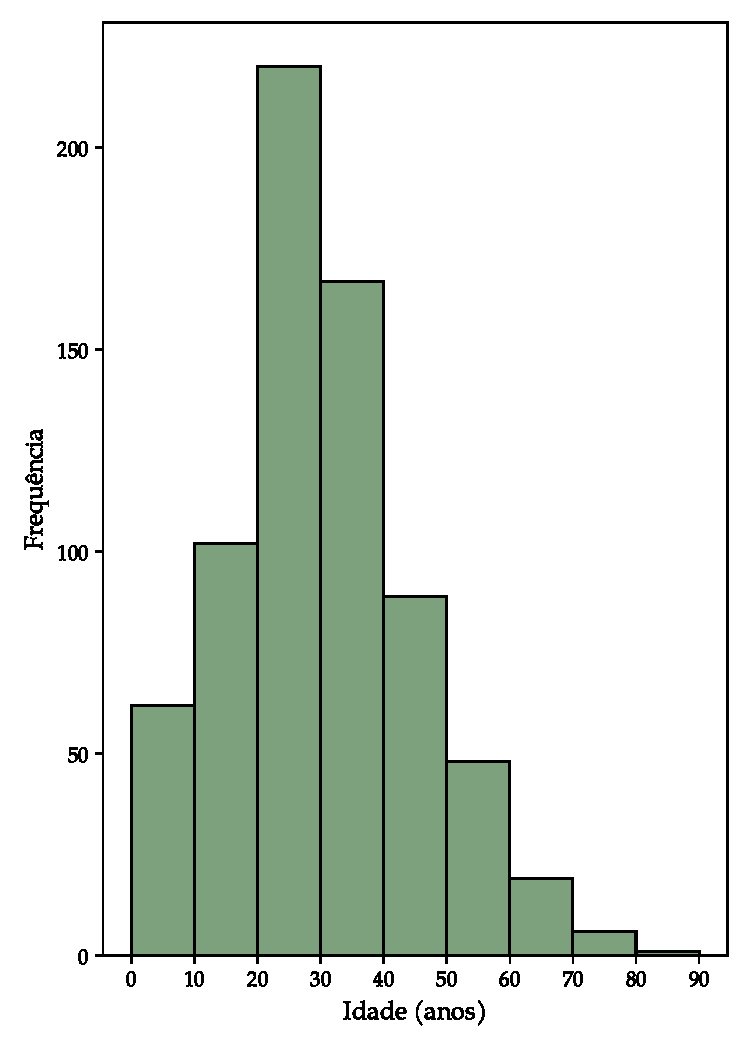
\includegraphics[width=\linewidth]{idade_histograma.pdf}
			\caption{Histograma}
		\end{subfigure}
		\hfill
		\begin{subfigure}[t]{.49\textwidth}
			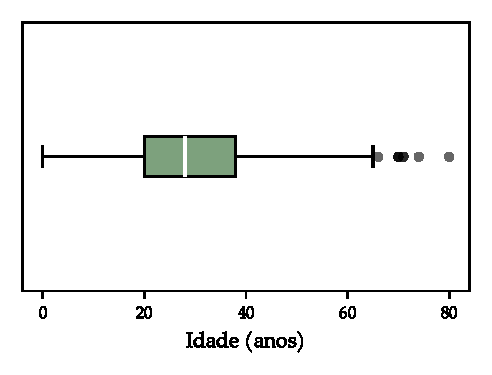
\includegraphics[width=\linewidth]{idade_boxplot.pdf}
			\caption{\emph{Boxplot}}
		\end{subfigure}
		\caption{Gráficos relativos às idades dos passageiros}
	\end{figure}
	O histograma ilustra uma distribuição unimodal com assimetria à direita, mostrando que $20 \vdash 30$ é a faixa etária mais frequente.
	
	O \emph{boxplot} também nos evidencia assimetria à direita. A começar, sua ``caixa'' nos informa que 50\% dos passageiros possuem entre 20 a 38 anos. Todavia, sua linha mediana (28 anos) está ligeiramente deslocada para baixo. Por fim, ele destaca a presença de \emph{outliers} à direita --- valores acima de seu ``bigode'' superior --- o que corresponde à minoria de passageiros idosos do Titanic.
	\begin{figure}[H]
		\centering
		\begin{subfigure}[t]{.49\textwidth}
			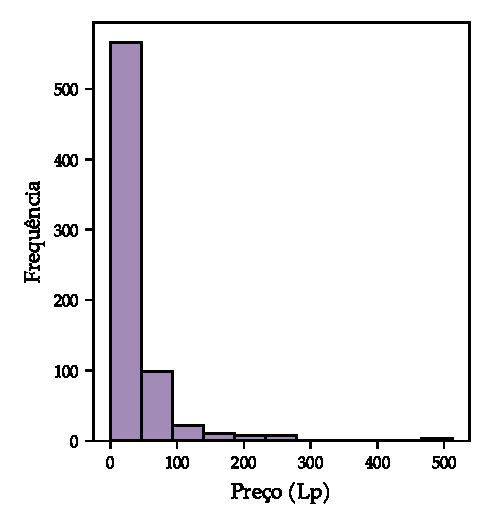
\includegraphics[width=\linewidth]{preco_histograma.pdf}
			\caption{Histograma}
		\end{subfigure}
		\hfill
		\begin{subfigure}[t]{.49\textwidth}
			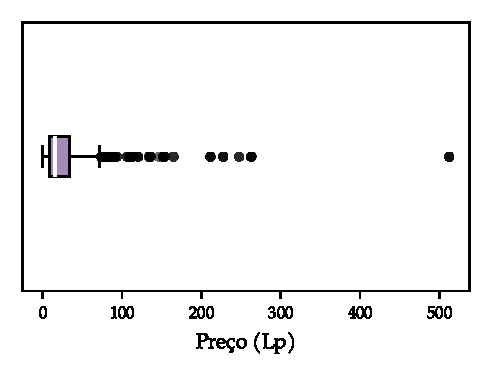
\includegraphics[width=\linewidth]{preco_boxplot.pdf}
			\caption{\emph{Boxplot}}
		\end{subfigure}
		\caption{Gráficos relativos aos preços dos bilhetes dos passageiros}
	\end{figure}
	Tanto o histograma, quanto o \emph{boxplot} indicam uma extrema assimetria à direita nos preços. No histograma, a primeira barra (bilhetes mais baratos) concentra quase todos os dados, enquanto as demais formam uma cauda longa e quase invisível.

	O \emph{boxplot}, por sua vez, apresenta não só uma linha mediana mais próxima de $Q_1$ do que $Q_3$, mas a ``caixa'' como um todo é muito estreita, seguida por uma longa sequência de \emph{outliers} à direita.

	Tal configuração faz sentido se considerarmos que a maioria dos passageiros viajaram em cabines simples, ao passo que alguns seletos alugaram cabines de luxo.
	
	% --- BIBLIOGRAFIA ---
	%\printbibliography
\end{document}
